\subsection{Dynamic scaling}

\begin{frame}
	\frametitle{Dynamic scaling framework for the round-trip}
	The asymptotic dynamic FSS behavior is obtained by taking 
	$t_s \to \infty$ and $L \to \infty\,$:
	\begin{eqnarray}
  		&K = w(t) L^{y_w}\,, \qquad &\Upsilon = t_s/L^{\zeta}\,,  
  		\label{KZscavar}\\
 		 &\Theta_i
 		 = w_i\, t_s^{1-\kappa} \,,\qquad &\Theta = w(t) \,
  		t_s^{1-\kappa} = t / t_s^{\kappa} \,,\nonumber
	\end{eqnarray}
	where
	\begin{eqnarray}
		\zeta = y_w + z\,,\qquad 
		\kappa = {z/\zeta} \,,\qquad
		1-\kappa = {y_w/\zeta}\,.\label{KZexps}
	\end{eqnarray}
	with $w_f = - w_i = w _\star$, we have:
	\begin{eqnarray}
  		\Upsilon = t_s/L^{\zeta}\,, \quad
  		\Theta = w(t) \, t_s^{1-\kappa}\,,\quad
  		\Theta_\star =  w_\star\, t_s^{1-\kappa} \,\,.
 		\label{scalvar2}
  	\end{eqnarray}
\end{frame}




\section{Numerical results}


\subsection{Classical Ising}

\begin{frame}
	%\frametitle{$\qquad \qquad \qquad M^{(a/b)}(t,t_s,w_\star,L) 
	%			\approx L^{-y_l} {\cal M}_i(\Upsilon,\Theta, \Theta_\star)$}
	\frametitle{Numerical results - Classical Ising}
	
	%\begin{align}
	%	M(t,t_s,w_i,L) \approx L^{-y_l} {\cal M}_i(\Upsilon,\Theta)\,\,.
	%\end{align}
	\begin{columns}
	\begin{column}{0.52\textwidth}
	\begin{figure}[!htb]
  		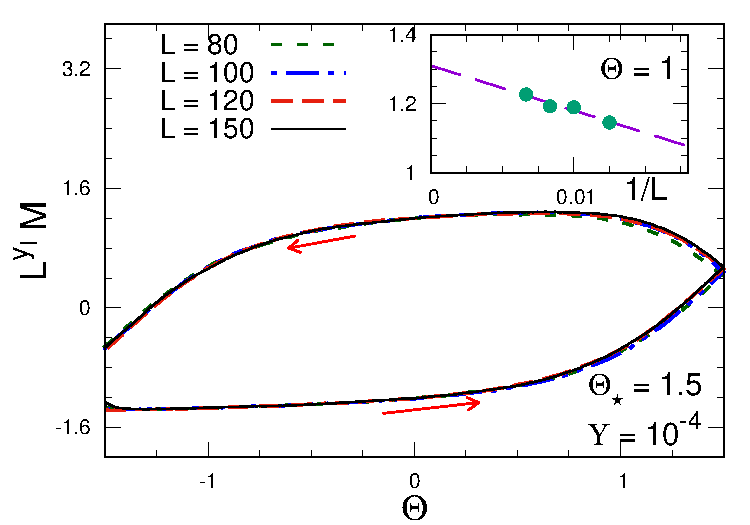
\includegraphics[width=1.\columnwidth]{paper/isC2DT15Y104.pdf}
  		
  		\caption{ \alert{$M^{(a/b)}(t,t_s,w_\star,L) 
				\approx L^{-y_l} {\cal M}_i(\Upsilon,\Theta, \Theta_\star)$}
				$\Upsilon=10^{-4}$, fixed $\Theta_\star =
    				1.5$ and plotted versus $\Theta=w(t) t_s^{1-\kappa}$.  }
  		\label{roundtripM}
	\end{figure}
	\end{column}
	\begin{column}{0.5\textwidth}
	
	\begin{figure}[!htb]
    		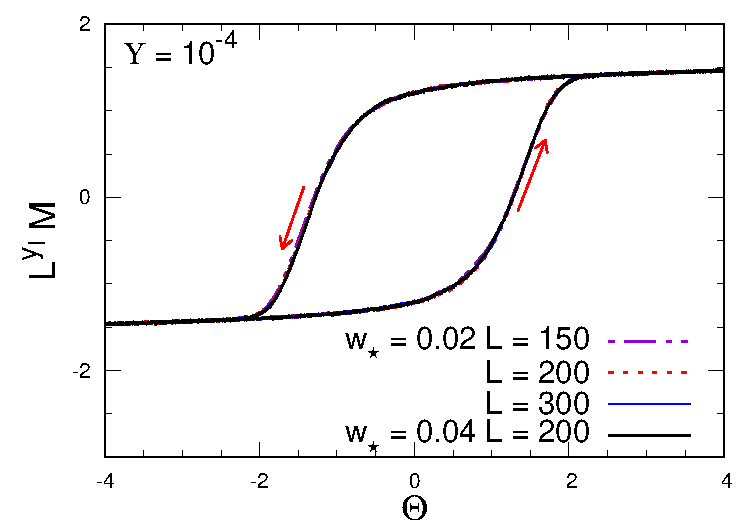
\includegraphics[width=1.\columnwidth]{paper/isC2Dw002Y104.pdf}
  		\caption{ Thermalized classical state for
    		fixed $\Upsilon=10^{-4}$, and fixed $w_\star = 0.02$ and $w_\star
    		= 0.04$. $\qquad \qquad \qquad \qquad \qquad \qquad \qquad \qquad$}
  		\label{roundtripMW}
	\end{figure}
	\end{column}
	\end{columns}
	
\end{frame}



\begin{comment}
\subsection{Quantum Ising}

\begin{frame}
	
	\frametitle{Numerical results - Quantum Ising}
	\begin{columns}
	\begin{column}{0.52\textwidth}
	\begin{figure}[!htb]
		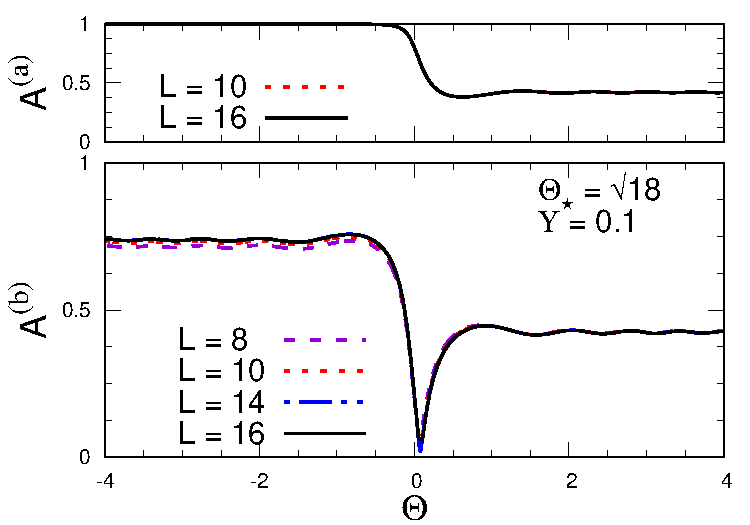
\includegraphics[width=1\columnwidth]{paper/headIQMY01ThA.pdf}
		\caption{ \alert{$ A^{(a/b)}(t,t_s,w_\star,L) \approx 
 				{\cal A}^{(a/b)}(\Upsilon,\Theta,\Theta_\star)\,\,$};
		fixed $\Upsilon = t_s/L^\zeta= 0.1$ and $\Theta_\star = w_\star
  		L^{1-\kappa}=\sqrt{18}$, for the outward (top) and return (bottom). }
    		\label{roundtripA}
	\end{figure}
	
	\end{column}
	\begin{column}{0.5\textwidth}
	
	\begin{figure}[!htb]
		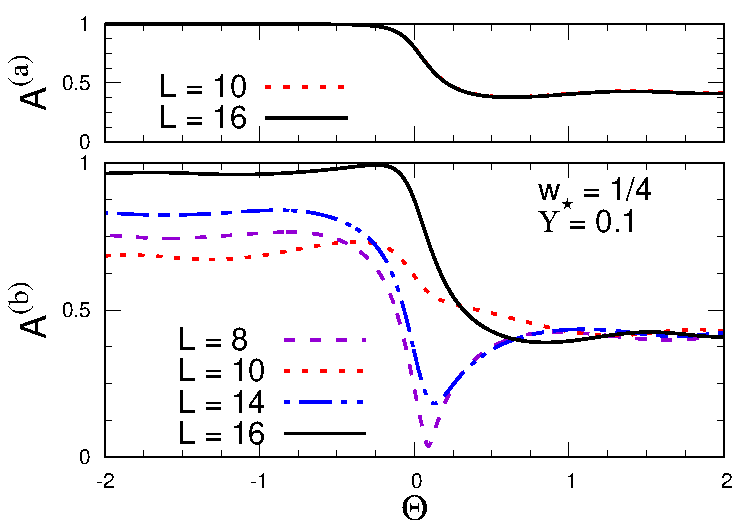
\includegraphics[width=1\columnwidth]{paper/headIQMY01W025A.pdf}
  		\caption{ Fixed $\Upsilon = 0.1$ and $w_\star = 1/4$, for the outward 
  		(top) and return (bottom), versus $\Theta=w(t)L^{1-\kappa}$.
  		$\qquad \qquad \qquad \qquad \qquad \qquad \qquad \qquad$}
  		\label{roundtripAW}
		\end{figure}
	\end{column}
	\end{columns}

\end{frame}
\end{comment}


\subsection{Kitaev chain}

\begin{frame}
	
	\frametitle{Numerical results - Kitaev chain}
	
	\begin{columns}
	\begin{column}{0.52\textwidth}
		\begin{figure}[!htb]
			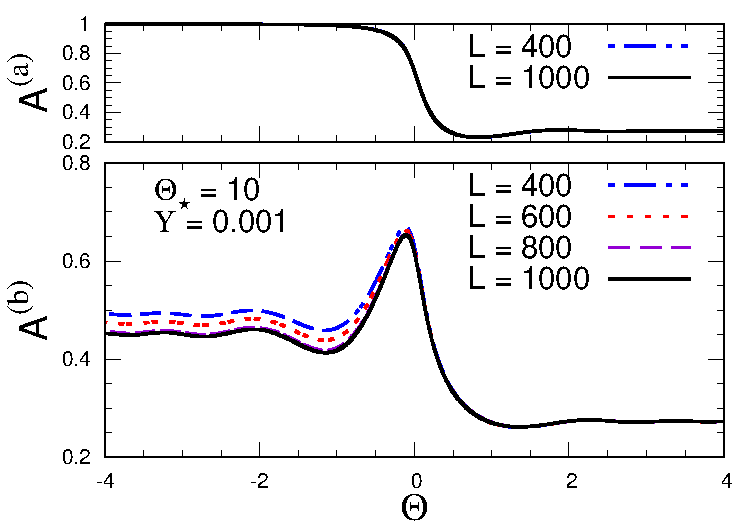
\includegraphics[width=1\columnwidth]{paper/headKITY0001Th10A.pdf}
  			\caption{ \alert{$ A^{(a/b)}(t,t_s,w_\star,L) \approx 
 				{\cal A}^{(a/b)}(\Upsilon,\Theta,\Theta_\star)\,\,$};
  			Finite $\Theta_\star=10$ at fixed $\Upsilon =t_s/L^\zeta = 0.001$
  			and $\Theta_\star = w_\star L^{1-\kappa}=10$, for outward
  			 and return.
    $\Theta$, }
  			\label{roundtripdfssE}
		\end{figure}
	
	\end{column}
	\begin{column}{0.5\textwidth}
	
	\begin{figure}[!htb]
  		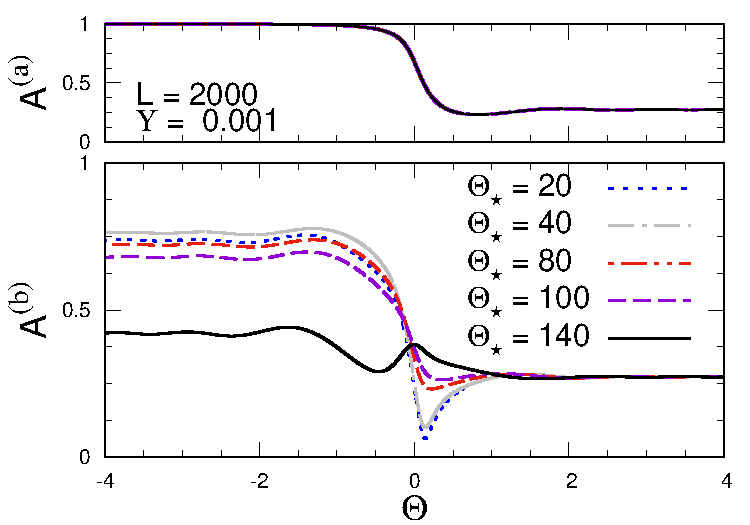
\includegraphics[width=1\columnwidth]{paper/headKITY0001L2000A.pdf}
 		\caption{At $L=2000$ and $\Upsilon = 0.001$ for the outward (top)
 		 and return (bottom), versus $\Theta$, for various 
 		 $\Theta_\star$. $\qquad \qquad \qquad \qquad \qquad \qquad \qquad \qquad \qquad \qquad \qquad \qquad \qquad \qquad \qquad \qquad$}
 		 %=w(t)L^{1-\kappa}
  \label{diffThetaStarA}
\end{figure}

	\end{column}
	\end{columns}


\end{frame}
